\chapter{Méthodologie et Conception du Système}
\label{chap:methodologie}

\section{Introduction}
Ce chapitre présente la méthodologie complète et la conception du système proposé pour estimer le \emph{temps de cuisson} (\(T_c\), en minutes) des haricots à partir d'images. Le système adopté est hybride et séquentiel : il repose sur deux modèles indépendants et spécialisés — un modèle de \textbf{classification} chargé d'identifier si l'image contient un haricot (et, le cas échéant, d'identifier sa variété parmi huit classes) et un modèle de \textbf{régression} chargé d'estimer le temps de cuisson lorsque l'image a été validée comme étant un haricot. Ce découpage vise à améliorer la robustesse opérationnelle (éviter des estimations sur des images hors-domaine), à optimiser l'utilisation des ressources embarquées (ne solliciter le modèle de régression que lorsque nécessaire) et à faciliter l'intégration TinyML sur plateformes contraintes (smartphone et microcontrôleur) \cite{warden2019,alirezazadeh2022cascade}.
L'architecture logicielle de la solution met ainsi en œuvre deux pipelines de prétraitement et deux modèles distincts, chacun optimisé et quantifié selon des objectifs différents : le modèle de classification est conçu pour être très léger et quantifié en INT8 (ex. MobileNetV2 quantifié post-training), tandis que le modèle de régression privilégie la précision et peut utiliser une quantification en float16 ou une quantification mixte selon les tests empiriques. La logique applicative (smartphone) orchestre l'enchaînement classification $\rightarrow$ décision $\rightarrow$ régression et l'affichage des résultats à l'utilisateur.
Dans la suite du chapitre, nous décrivons les jeux de données (séparés pour classification et régression), l'analyse exploratoire, le protocole de prétraitement distinct pour chaque tâche, les architectures testées, le workflow d'entraînement et d'optimisation TinyML, ainsi qu'une comparaison chiffrée et une discussion critique des choix adoptés.

\section{Vue d'ensemble du pipeline proposé}

\begin{figure}[H]
	\centering
	\small
	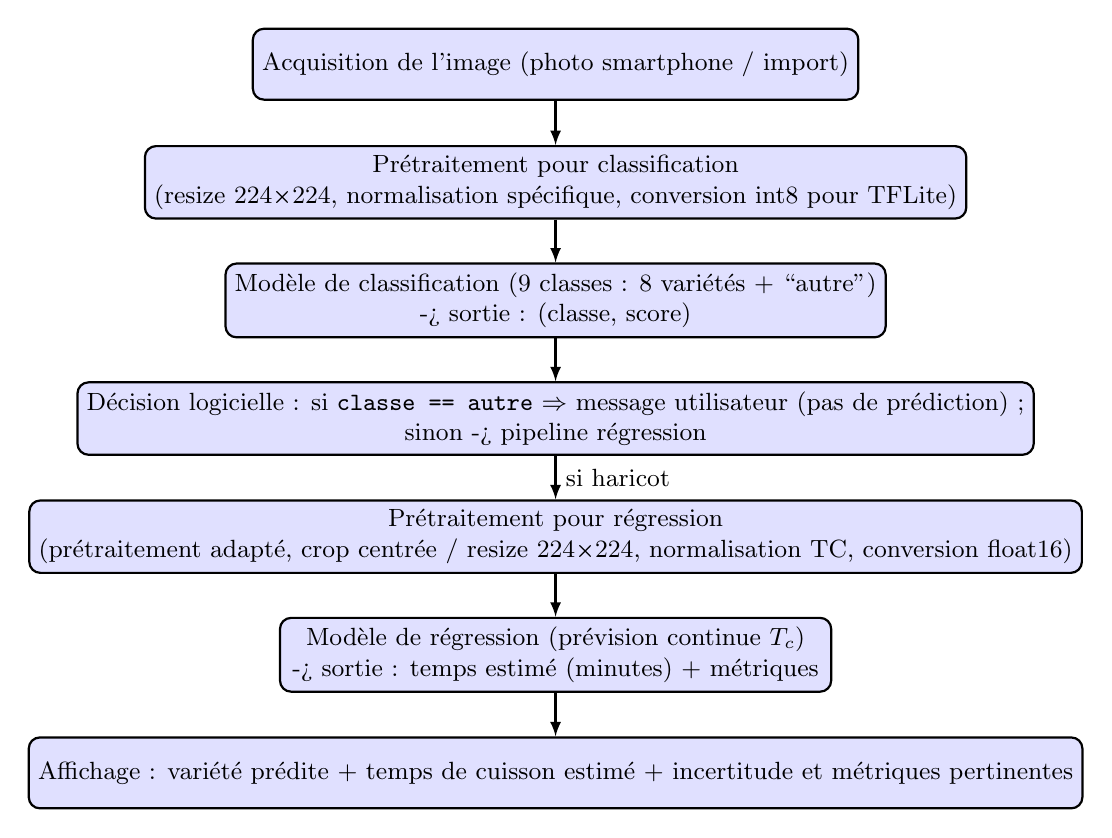
\begin{tikzpicture}[node distance=1.5cm, >=latex, thick, font=\small]
		\tikzstyle{bloc} = [rectangle, draw=black, fill=blue!12, rounded corners, minimum width=7.0cm, minimum height=0.9cm, align=center]
		\node[bloc] (acq) {Acquisition de l'image (photo smartphone / import)};
		\node[bloc, below of=acq] (pre_cl) {Prétraitement pour classification \\ (resize 224×224, normalisation spécifique, conversion int8 pour TFLite)};
		\node[bloc, below of=pre_cl] (classif) {Modèle de classification (9 classes : 8 variétés + ``autre'') \\ -> sortie : (classe, score)};
		\node[bloc, below of=classif] (decision) {Décision logicielle : si \texttt{classe == autre} $\Rightarrow$ message utilisateur (pas de prédiction) ;\\ sinon -> pipeline régression};
		\node[bloc, below of=decision] (pre_reg) {Prétraitement pour régression \\ (prétraitement adapté, crop centrée / resize 224×224, normalisation TC, conversion float16)};
		\node[bloc, below of=pre_reg] (reg) {Modèle de régression (prévision continue $T_c$) \\ -> sortie : temps estimé (minutes) + métriques};
		\node[bloc, below of=reg] (aff) {Affichage : variété prédite + temps de cuisson estimé + incertitude et métriques pertinentes};
		\draw[->] (acq) -- (pre_cl);
		\draw[->] (pre_cl) -- (classif);
		\draw[->] (classif) -- (decision);
		\draw[->] (decision) -- node[right]{si haricot} (pre_reg);
		\draw[->] (pre_reg) -- (reg);
		\draw[->] (reg) -- (aff);
	\end{tikzpicture}
	\caption{Pipeline global du système : classification suivie (si nécessaire) d'une régression.}
	\label{fig:pipeline_global}
\end{figure}

\subsection{Dataset de classification (\(\mathcal{D}_{\text{clf}}\))}

\begin{itemize}
	\item \textbf{Composition} : 9 classes — huit variétés de haricots, chacune subdivisée en 7 sous-variétés (soit \(8 \times 7 = 56\) sous-classes), et une classe supplémentaire \texttt{``autre''}. Chaque sous-variété contient 200 images, soit \(56 \times 200 = 11\,200\) images pour les haricots. La classe \texttt{``autre''} regroupe 1\,000 images issues d’objets divers (chien, chat, voiture, personne, etc.), extraites du dataset libre \emph{Common Objects in Context (COCO)} \cite{lin2014microsoft}. Ces 1\,000 images constituent un échantillon du split validation original du dataset COCO, qui en contient 5\,000.
	\item \textbf{Taille totale} : 12\,200 images (11\,200 images de haricots + 1\,000 images de la classe \texttt{``autre''}).
	\item \textbf{Splits} :
	      \begin{itemize}
		      \item Entraînement/validation : 190 images par sous-variété (soit \(190 \times 56 = 10\,640\)) + 800 images de la classe \texttt{``autre''}, réparties selon une proportion 80/20.
		      \item Test : 10 images par sous-variété (soit \(10 \times 56 = 560\)) + 200 images de la classe \texttt{``autre''}.
	      \end{itemize}
	\item \textbf{Format} : images RGB redimensionnées en 224×224 pixels pour l’entraînement; métadonnées associées : label de classe, label de sous-varieté, et identifiant d’image.
	\item \textbf{Augmentation} : aucune stratégie d’augmentation n’a été appliquée sur ce jeu de données.
	\item \textbf{Problèmes identifiés} : variation de résolution et d’éclairage entre les sources d’images; risque de confusion inter-sous-variétés de haricots du fait de similarités visuelles; distribution hétérogène entre classes spécifiques et la classe \texttt{``autre''}.
\end{itemize}


\subsection{Dataset de régression (\(\mathcal{D}_{\text{reg}}\))}

Le second jeu de données est dédié à la tâche de régression visant à prédire le temps de cuisson (\(T_c\), exprimé en minutes) des haricots.

\begin{itemize}
	\item \textbf{Composition} : il comprend \(\mathbf{8}\) variétés de haricots (identiques à celles présentes dans \(\mathcal{D}_{\text{clf}}\), à l’exception de la classe \texttt{``autre''}). Le dataset totalise \(\mathbf{11\,200}\) images couleur, réparties uniformément avec \(\mathbf{1\,400}\) images par variété.
	\item \textbf{Annotation} : chaque image est associée à une mesure expérimentale du temps de cuisson \(T_c\), déterminée selon le critère culinaire \emph{fork-tender} \cite{hall2017beanquality}. Une incertitude expérimentale estimée à \(\pm 1\) minute (variabilité opérateur et conditions de cuisson) est attachée à chaque échantillon.
	\item \textbf{Splits} : les données ont été séparées selon un ratio \(80/10/10\) en ensembles d’entraînement, validation et test, avec une seed fixe de \textbf{42} pour assurer la reproductibilité. Afin de respecter la distribution des temps de cuisson par variété, une stratification par quantiles de \(T_c\) a été appliquée, comme recommandé dans des contextes de régression hétérogène \cite{guyon2017analysis}.
	\item \textbf{Augmentation} : pour accroître la robustesse et réduire le risque de sur-apprentissage, seules les images d’entraînement ont subi des transformations de data augmentation (flips horizontaux et verticaux, mise à l’échelle, zoom aléatoire). Un facteur global de multiplication \(\times 5\) a ainsi été obtenu.
	\item \textbf{Prétraitement} : toutes les images ont été redimensionnées en 224×224 pixels. Contrairement aux pratiques standards de normalisation des intensités dans \([0,1]\) \cite{lecun2015deep}, les images ont été conservées dans l’espace d’origine \([0,255]\) afin de réduire la taille des fichiers sauvegardés (au format HDF5). La normalisation est réalisée dynamiquement au moment du chargement en mémoire, ce qui optimise le compromis entre efficacité de stockage et préparation des données pour l’entraînement.
	\item \textbf{Normalisation des labels} : les temps de cuisson bruts variaient initialement dans l’intervalle \([51, 410]\) minutes. Pour stabiliser l’entraînement et accélérer la convergence des modèles, une normalisation Min–Max a été appliquée :
	      \[
		      T_c^{\text{norm}} = \frac{T_c - T_{\min}}{T_{\max} - T_{\min}}, \quad T_{\min} = 51, \; T_{\max} = 410.
	      \]
	      Ainsi, les labels sont projetés dans \([0,1]\). Ce choix est cohérent avec la littérature, la mise à l’échelle linéaire facilitant l’optimisation dans les réseaux de neurones et réduisant les effets liés à la différence d’échelle entre variables \cite{bishop2006pattern}.
	\item \textbf{Observation} : la distribution des temps de cuisson est multimodale et fortement hétérogène entre variétés, certaines ayant une cuisson moyenne relativement courte (proches de 60 minutes), d’autres beaucoup plus longue (supérieure à 300 minutes). Ces caractéristiques influencent le biais de prédiction et rendent la tâche particulièrement complexe.
\end{itemize}

\begin{figure}[H]
	\centering
	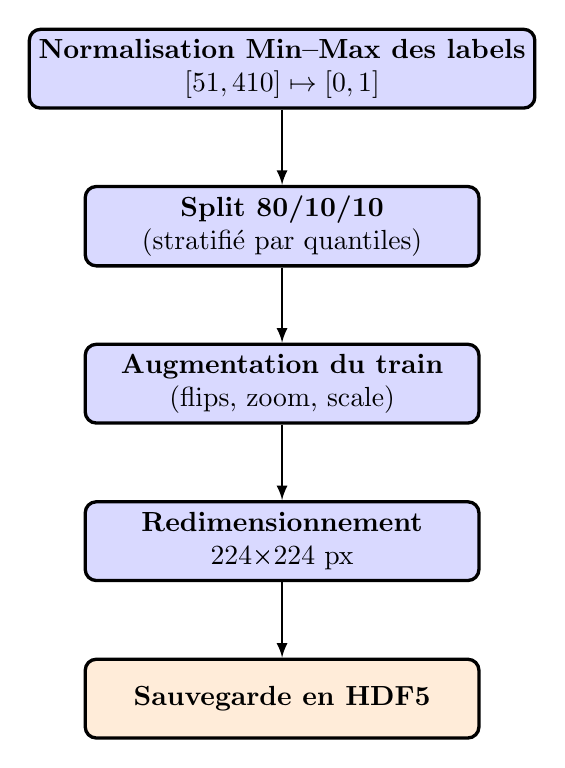
\begin{tikzpicture}[
			node distance=2cm,
			>=latex,
			box/.style={
					rectangle,
					rounded corners=4pt,
					draw=black,
					very thick,
					minimum width=5cm,
					minimum height=1cm,
					align=center
				},
			dataset/.style={box, fill=green!15},
			process/.style={box, fill=blue!15},
			storage/.style={box, fill=orange!15}
		]

		% Nodes
		\node[process] (labels) {\textbf{Normalisation Min–Max des labels} \\ \([51,410] \mapsto [0,1]\)};
		\node[process, below of=labels] (split) {\textbf{Split 80/10/10} \\ (stratifié par quantiles)};
		\node[process, below of=split] (augmentation) {\textbf{Augmentation du train} \\ (flips, zoom, scale)};
		\node[process, below of=augmentation] (resize) {\textbf{Redimensionnement} \\ 224×224 px};
		\node[storage, below of=resize] (hdf5) {\textbf{Sauvegarde en HDF5}};

		% Arrows
		\draw[->, thick] (labels) -- (split);
		\draw[->, thick] (split) -- (augmentation);
		\draw[->, thick] (augmentation) -- (resize);
		\draw[->, thick] (resize) -- (hdf5);

	\end{tikzpicture}
	\caption{Pipeline de préparation du dataset de régression.}
	\label{fig:dataset_reg_pipeline}
\end{figure}

\subsection{Justification du découpage en deux jeux distincts}

La séparation en deux jeux de données distincts (\(\mathcal{D}_{\text{clf}}\) pour la classification et \(\mathcal{D}_{\text{reg}}\) pour la régression) repose sur plusieurs considérations conceptuelles et pratiques :
\begin{enumerate}
	\item \textbf{Sécurité et validité des prédictions} : lors de l'acquisition, des images hors-catégorie (objets non pertinents ou bruit visuel) peuvent être présentes. Entraîner directement un modèle de régression sur de telles images conduirait à des prédictions aberrantes ou hors domaine \cite{zhang2018generalized}. L'utilisation d'un modèle de classification préalable permet de filtrer les entrées et de garantir que la régression est appliquée uniquement sur des images pertinentes, améliorant ainsi la robustesse du système.

	\item \textbf{Différences méthodologiques et d'optimisation} : les tâches de classification et de régression diffèrent par leurs objectifs et contraintes. La classification repose sur un objectif catégoriel (cross-entropy ou focal loss), tandis que la régression vise à prédire une variable continue (\(T_c\)) avec des fonctions de perte telles que MSE ou MAE \cite{goodfellow2016deep}. Ces différences impliquent des prétraitements distincts, des augmentations adaptées, et des stratégies de normalisation ciblées pour stabiliser l’entraînement \cite{lecun2015deep}. Traiter les deux tâches séparément permet d’optimiser finement chaque pipeline sans compromis sur la performance.

	\item \textbf{Contraintes liées aux systèmes embarqués et à la quantification} : dans un contexte TinyML, la politique de quantification et d’optimisation peut diverger selon la tâche. Les modèles de classification peuvent être fortement quantifiés en INT8 pour réduire la latence et la consommation énergétique, tandis que la régression, nécessitant souvent plus de précision, peut exploiter une quantification plus douce (float16 ou mixte) \cite{han2020tinyml}. Séparer les pipelines permet donc d’adapter la compression et l’optimisation à chaque objectif.
\end{enumerate}

Cette approche modulaire, consistant à découpler la classification et la régression, est largement adoptée dans la littérature sur les systèmes de vision embarquée et la détection d’objets complexes \cite{redmon2016you,liu2016ssd}.


\section{Analyse exploratoire (EDA) et statistiques descriptives}

Cette section résume les analyses réalisées sur \(\mathcal{D}_{\text{reg}}\) et \(\mathcal{D}_{\text{clf}}\), et met en évidence les implications pour la modélisation.

\subsection{Synthèse statistique pour la régression}

Le tableau \ref{tab:stats_descriptives} (extrait et adapté) compile les principales statistiques par variété (moyenne, écart-type, min, max, effectif). Les résultats confirment la forte hétérogénéité inter-variétés : la moyenne de \(T_c\) varie de \(\approx 118.9\) min à \(\approx 237.4\) min tandis que les variances s'étendent largement, notamment pour la variété \texttt{Macc55}.

\begin{table}[H]
	\centering
	\caption{Statistiques descriptives des temps de cuisson ($T_c$ en minutes) par variété (extrait).}
	\label{tab:stats_descriptives}
	\begin{tabular}{lccccc}
		\toprule
		\textbf{Variété} & \textbf{Moyenne ($\mu$)} & \textbf{Écart-type ($\sigma$)} & \textbf{Min} & \textbf{Max} & \textbf{Effectif} \\ \midrule
		Dor701           & 145.86                   & 72.67                          & 62           & 280          & 1400              \\
		Escapan021       & 159.00                   & 77.47                          & 65           & 287          & 1400              \\
		GPL190C          & 160.00                   & 74.19                          & 70           & 295          & 1400              \\
		GPL190S          & 144.57                   & 66.65                          & 58           & 270          & 1400              \\
		Macc55           & 237.43                   & 103.99                         & 88           & 410          & 1400              \\
		NIT4G16187       & 118.86                   & 45.18                          & 68           & 210          & 1400              \\
		Senegalais       & 155.71                   & 78.38                          & 70           & 300          & 1400              \\
		TY339612         & 148.14                   & 77.85                          & 51           & 286          & 1400              \\ \bottomrule
	\end{tabular}
\end{table}

\paragraph{Implications}
\begin{itemize}
	\item Les variétés à forte variance (ex. \texttt{Macc55}) exigeront un modèle capable de capturer une large palette d'apparences visuelles ; l'erreur absolue moyenne (MAE) attendue sera plus élevée pour ces classes.
	\item Une normalisation Min--Max globale des cibles est possible, mais on doit considérer l'utilisation d'une normalisation par-varieté ou l'introduction d'un embedding de variété (si la variété est connue) pour améliorer la performance locale.
\end{itemize}

\subsection{Analyse du dataset de classification}

L'analyse exploratoire du dataset \(\mathcal{D}_{\text{clf}}\) met en évidence plusieurs points importants :

\begin{itemize}
	\item \textbf{Qualité des images} : toutes les images ont été vérifiées, et aucune image corrompue ou illisible n’a été détectée, garantissant la fiabilité des données pour l’entraînement.
	\item \textbf{Distribution des classes} : le dataset contient 9 classes — 8 variétés de haricots et une classe \texttt{autre} issue d’un échantillon du dataset COCO \cite{lin2014microsoft}. Chaque variété comprend 7 sous-variétés avec 190 images chacune, soit 1 400 images par variété. La classe \texttt{autre} contient 1 000 images diverses (chien, chat, voiture, personne, etc.), ce qui représente un choix volontaire pour refléter la proportion réaliste d’images hors-catégorie.
	\item \textbf{Variabilité visuelle} : des différences de luminosité, de contraste et de résolution entre sous-variétés ont été observées, justifiant l’usage futur d’augmentations photométriques pour améliorer la robustesse du modèle \cite{shorten2019survey}.
\end{itemize}

\subsection{Stratégie adoptée pour la classe \texttt{autre}}

Bien que la classe \texttt{autre} soit plus petite que les autres classes, cette répartition est \textbf{intentionnelle} afin de reproduire la proportion réaliste d’images hors-catégorie :

\begin{itemize}
	\item La classe \texttt{autre} est conservée telle quelle pour entraîner le modèle à détecter et rejeter les images hors-domaine.
	\item Une validation croisée stratifiée est utilisée pour évaluer la performance sur toutes les classes, y compris \texttt{autre}, afin de s’assurer que la taille réduite ne nuit pas à la capacité de généralisation \cite{buda2018systematic}.
\end{itemize}


\section{Architectures modèles et justification}

Nous testons deux familles de modèles : (i) architectures conçues ad hoc (CNN-1 / CNN-2) et (ii) modèles mobiles pré-entraînés (MobileNetV2, EfficientNet-B0, NASNetMobile). Les configurations et motivations restent proches de celles décrites précédemment ; nous rappelons ici les décisions liées au couplage classification / régression.

\subsection{Modèle de classification}

\begin{itemize}
	\item \textbf{Backbone recommandé} : MobileNetV2 (1.0, 224) fine-tuné sur \(\mathcal{D}_{\text{clf}}\). Raisons : excellente performance/empreinte mémoire, blocs inverted-residual favorables à la quantification INT8 et historique d'utilisation mobile \cite{sandler2018mobilenetv2}.
	\item \textbf{Sortie} : softmax 9 unités (8 variétés + \texttt{autre}).
	\item \textbf{Fonction de perte} : categorical cross-entropy avec éventuelle pondération de classes (class weights) pour corriger le déséquilibre.
	\item \textbf{Métriques} : accuracy globale, F1-score macro (pour tenir compte du déséquilibre), recall/precision par classe, matrice de confusion. (Les définitions formelles des métriques sont détaillées dans la revue de littérature.)
	\item \textbf{Optimisations} : PTQ int8; si dégradation trop forte, utiliser QAT.
\end{itemize}

\subsection{Modèle de régression}

\begin{itemize}
	\item \textbf{Backbones testés} : CNN personnalisé (CNN-1 / CNN-2), EfficientNet-B0 (fine-tuning) selon compromis précision/taille. Le modèle final sélectionné dans les expériences précédentes a été un CNN personnalisé entraîné from-scratch et plus simple (cf. rapport d'entraînement).
	\item \textbf{Sortie} : une seule unité pour la régression continue (valeur normalisée $\tilde{y}$).
	\item \textbf{Fonction de perte} : MSE (principal), suivi de MAE/MAPE comme métriques secondaires et critères d'arrêt; suivi de \(R^2\) pour évaluer la part de variance expliquée.
	\item \textbf{Optimisations} : quantification float16 pour préserver la précision numérique; PTQ int8 testé avec calibration pour mesurer impact.
\end{itemize}

\section{Workflow d'entraînement, conversion et évaluation}

\subsection{Procédure d'entraînement reproductible}

Pour chaque modèle (classification et régression) :
\begin{enumerate}
	\item Préparer HDF5 (ou TFRecord) par split avec seed fixe (reproductibilité).
	\item Appliquer les augmentations et normalisations correspondantes selon le pipeline.
	\item Entraîner avec Adam (baseline) : $\mathrm{lr}=10^{-4}$, batch size = 32 (ajuster selon VRAM), scheduler (Cosine ou ReduceOnPlateau), early stopping (patience 5 sur validation loss). Epochs baseline = 100.
	\item Logger via TensorBoard, sauvegarder checkpoints, et conserver le meilleur modèle sur la validation.
\end{enumerate}

\subsection{Conversion et quantification TFLite}

\begin{itemize}
	\item \textbf{Classification} : conversion PTQ INT8 avec dataset de calibration (subset representatif). Si la performance chute de plus de X\% (seuil à définir empiriquement), exécuter QAT quelques epochs puis reconvertir.
	\item \textbf{Régression} : conversion float16 par défaut ; tester PTQ int8 en gardant un set de test calibrant pour estimer la dégradation MAE/RMSE.
\end{itemize}

\subsection{Évaluation finale et mesures embarquées}

Mesures à effectuer sur la plateforme cible (smartphone Android API≥24) :
\begin{itemize}
	\item \textbf{Taille binaire} (.tflite) avant/après quantification.
	\item \textbf{Latence} d'inférence (cold start, warm runs), percentiles 50/90/99 sur N exécutions.
	\item \textbf{Consommation énergétique} par inférence (si instrumentation possible).
	\item \textbf{Concordance} entre sortie du modèle float32 de référence et sortie TFLite (tolerance MAE).
\end{itemize}

\section{Intégration dans l'application mobile et UX}

Au niveau applicatif (smartphone Android), le fonctionnement est le suivant :

\begin{enumerate}
	\item L'utilisateur capture ou charge une image.
	\item L'image subit le pipeline \(\mathcal{P}_{\text{clf}}\) puis passe au modèle de classification quantifié INT8.
	\item Si le modèle prédit la classe \texttt{autre} avec confiance supérieure à un seuil \(s_{\text{rej}}\) (ex. 0.6), l'application affiche un message : \emph{``L'application ne prédit le temps de cuisson que pour des images de haricots. Veuillez fournir une photo claire d'un haricot.''}
	\item Si le modèle prédit une des 8 variétés avec confiance suffisante, l'application déclenche le pipeline \(\mathcal{P}_{\text{reg}}\) (prétraitement pour régression) et exécute le modèle de régression (float16).
	\item L'interface affiche : la \textbf{variété} prédite (avec score), le \textbf{temps estimé $T_c$} (minutes) retransformé depuis l'échelle normalisée, et une estimation d'intervalle d'incertitude (ex. $\pm$ MAE sur la variété si disponible). Les métriques globales (acc, F1 pour la classification; MAE, RMSE pour la régression) sont accessibles dans une section ``Plus d'infos'' pour les utilisateurs techniques.
\end{enumerate}

\paragraph{Gestion des seuils et de la confiance}
Il est recommandé d'ajouter un mécanisme de rejet (thresholding) pour éviter d'exécuter la régression si la confiance de classification est basse. De plus, enregistrer ces exemples faibles en confidence pour une future annotation manuelle permettra d'améliorer le dataset (active learning).

\section{Discussion critique et limites}

\subsection{Points forts}
\begin{itemize}
	\item \textbf{Robustesse opérationnelle} : la classification préalable évite des prédictions aberrantes hors-domaine.
	\item \textbf{Efficacité embarquée} : quantification et architecture mobile permettent une exécution locale rapide et à faible consommation.
	\item \textbf{Séparabilité des responsabilités} : deux modèles spécialisés facilitent le débogage, la maintenance et la mise à jour incrémentale.
\end{itemize}

\subsection{Limites et pistes d'amélioration}
\begin{itemize}
	\item \textbf{Déséquilibre de la classe ``autre''} : risque de sur-apprentissage sur cette classe ; contraindre le modèle avec des pénalités de classe et enrichir la variété d'exemples hors-domaine.
	\item \textbf{Variabilité inter-variétés} : certaines variétés à forte variance (ex. \texttt{Macc55}) limitent la précision de la régression ; solutions : entraînement par-varieté, modèles spécialisés, ajout de métadonnées (humidité, conditions de stockage) si disponibles.
	\item \textbf{Quantification pour la régression} : int8 peut être trop agressif pour les tâches régressives ; float16 est souvent un bon compromis mais augmente légèrement la taille.
	\item \textbf{Mesures matérielles nécessaires} : latence et consommation doivent être mesurées sur divers appareils (CPU-only, NNAPI, GPU delegate) pour formuler des recommandations pratiques.
\end{itemize}

\section{Bonnes pratiques et recommandations pour la reproductibilité}

\begin{itemize}
	\item Consigner les seeds aléatoires pour la génération des splits et les augmentations.
	\item Exporter les artefacts (HDF5/TFRecord, checkpoints, scripts d'entraînement, scripts de conversion TFLite).
	\item Tester les modèles TFLite sur une suite d'appareils cibles pour mesurer latence et mémoire.
	\item Intégrer des tests unitaires comparant prédictions numpy/TF/Keras vs TFLite (tolerance MAE).
\end{itemize}

\section{Conclusion du chapitre}

Ce chapitre a présenté une méthodologie complète et reproductible pour la conception d'un système hybride \emph{classification $\rightarrow$ régression} destiné à prédire le temps de cuisson des haricots à partir d'images. La séparation des jeux de données et des pipelines de prétraitement, l'usage d'un modèle de classification quantifié INT8 pour filtrer le domaine, et d'un modèle de régression optimisé pour la précision (float16) constituent l'ossature de la proposition. Les choix techniques (architectures, augmentations, stratégies de quantification) sont motivés par un compromis précision/latence adapté aux contraintes embarquées. Le chapitre suivant (Implémentation) détaillera les scripts Keras/TensorFlow, les commandes de conversion TFLite (PTQ / QAT), les détails d'entraînement (callbacks, scheduler) et présentera les résultats empiriques complets (MAE, RMSE, R², matrices de confusion, latence et consommation mesurées).

